% Presentation
\documentclass{beamer}
% Styling
\usetheme{Frankfurt}
% Packages
\usepackage{hyperref}
\usepackage[utf8]{inputenc} % this is needed for german umlauts
\usepackage[english]{babel} % this is needed for german umlauts
\usepackage[T1]{fontenc}    % this is needed for correct output
                            % of umlauts in pdf
\usepackage{mathtools}      % maths
\setbeamerfont{myTOC}{series=\bfseries,size=\normalsize}
\AtBeginSection[]{\frame{\frametitle{Outline}%
                  \usebeamerfont{myTOC}\tableofcontents[current]}}

% Document
\begin{document}
% Metadata & cover
\title{Development of a payment channel over the Bitcoin network}
\subtitle{Final degree project}
\author{David Lozano Jarque <bitcoin@davidlj95.com>}
\date{5\textsuperscript{th} July 2017}
\subject{Computer Science}
\titlegraphic{
\includegraphics[width=\textwidth,height=.5\textheight,keepaspectratio]{img/bitcoin_logo.png}}
% Cover slide
\frame{\titlepage}
% Introduction
\section{Introduction}
% % What is Bitcoin: First apperance
\subsection{What is Bitcoin}
\begin{frame}{Bitcoin's appearance}
 \begin{block}{The creator}
  Satoshi Nakamoto @ Cryptography (\url{metzdowd.com})\\
  November 1\textsuperscript{st}, 2008
 \end{block}
 \begin{columns}
  \begin{column}{0.5\textwidth}
   \begin{center}
    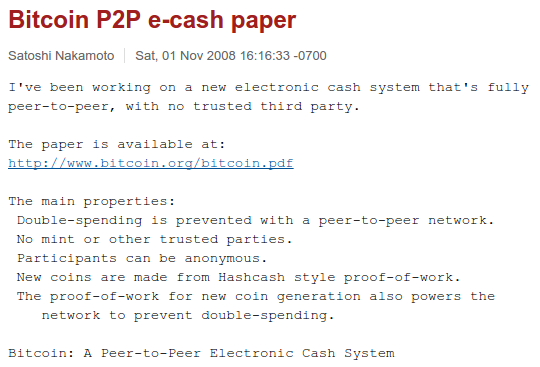
\includegraphics[width=\textwidth, height=0.8\textheight, keepaspectratio]{img/metzdowd_post.png}
   \end{center}
  \end{column}
  \begin{column}{0.5\textwidth}
   \begin{center}
    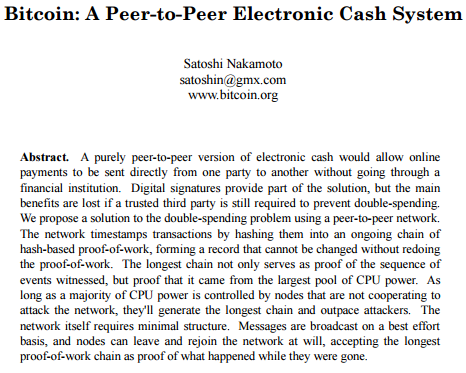
\includegraphics[width=\textwidth, height=0.8\textheight, keepaspectratio]{img/bitcoin_paper.png}
   \end{center}
  \end{column}
 \end{columns}
\end{frame}
% % What is Bitcoin: main specs
\begin{frame}{Bitcoin's definition}
 \begin{block}{Definition of Bitcoin}
  P2P network that allows payments between users without a trusted third
  party
 \end{block}
 \pause
 \begin{block}{Features}
  \begin{itemize}[<+->]
   \item Public ledger of transactions
   \item Public ledger using \textit{blockchain} technology
   \item Consensus via \textit{proof-of-work} algorithm
   \item Cryptography-enforced (digital ECDSA signatures \& hash functions)
   \item No trusted 3rd party (Pure P2P)
  \end{itemize}
 \end{block}
\end{frame}
% % How does bitcoin work
\subsection{How does Bitcoin work?}
\begin{frame}
 \begin{center}
  \textbf{How do we move currency?}
 \end{center}
\end{frame}
% % % Transactions
\begin{frame}{Transactions}
 \begin{block}{What is a Bitcoin transaction?}
  Message specifying the transfer of currency units (called \textit{bitcoins})
 \end{block}
 \pause
 \begin{block}{Transaction fields}
  A transaction moves currency units given an input to a new output
  \begin{itemize}[<+->]
   \item \texttt{version}
   \item \textbf{\texttt{inputs}}
   \item \textbf{\texttt{outputs}}
   \item \texttt{locktime}
  \end{itemize}
 \end{block}
 \pause
 \begin{exampleblock}{Basic Bitcoin transaction}
  \begin{center}
   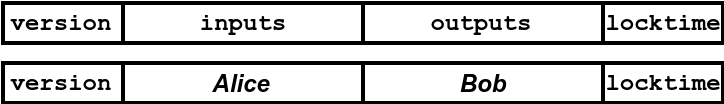
\includegraphics[width=\textwidth, height=0.8\textheight, keepaspectratio]{img/basic_tx.png}
  \end{center}
 \end{exampleblock}
\end{frame}
% % % Blocks
\begin{frame}
 \begin{center}
  \textbf{Where do we store transactions?}
 \end{center}
\end{frame}
\begin{frame}{Blocks}
 \begin{block}{What is a Bitcoin block?}
  Collection of transactions
 \end{block}
 \pause
 \begin{exampleblock}{Basic Bitcoin block}
  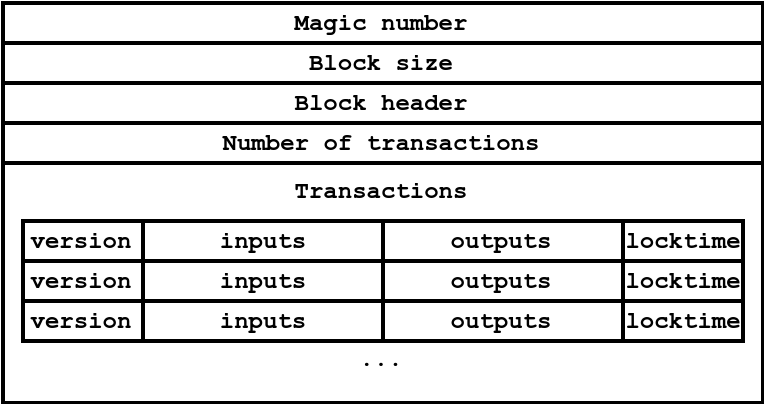
\includegraphics[width=\textwidth, height=0.8\textheight, keepaspectratio]{img/basic_block.png}
 \end{exampleblock}
\end{frame}
% % % Blockchain
\begin{frame}
 \begin{center}
  \textbf{Where do we store blocks?}
 \end{center}
\end{frame}
\begin{frame}{\textit{Blockchain}}
 \uncover<1-2>{
  \begin{block}{Bitcoin's \textit{blockchain}}
   Distributed and replicated database containing a collection of blocks, each one linked to the previous one using \textbf{their hashes} forming \textbf{a chain}
  \end{block}}
 \only<2>{
  \begin{exampleblock}{Basic Bitcoin's \textit{blockchain}}
   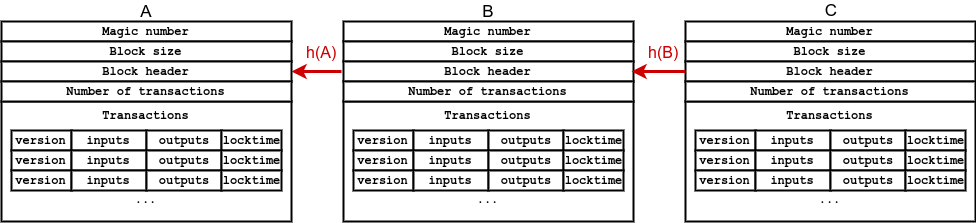
\includegraphics[width=\textwidth, height=0.8\textheight, keepaspectratio]{img/basic_blockchain.png}
  \end{exampleblock}}
 \only<3>{
  \begin{block}{Rewards}
   Appending a new block to the chain is rewarded with \textbf{newly generated currency units} with a \textit{no-input} transaction called
   a \textbf{generation transaction}
  \end{block}}
\end{frame}
% % % Consensus
\begin{frame}
 \begin{center}
  \textbf{Who decides who can create next block?}
 \end{center}
\end{frame}
\begin{frame}{Consensus}
 \begin{block}{\textit{Proof-of-work}}
  Piece of data difficult to generate but easy to verify it meets certain
  requirements
 \end{block}
 \pause
 \begin{block}{Bitcoin's \textit{proof-of-work}}
  Field in block's header must contain a hash of the block itself whose
  value \textbf{is less than a dynamically adjusted value}
 \end{block}
\end{frame}
\begin{frame}{\textit{Proof-of-work}}
 \begin{exampleblock}{Basic Bitcoin's \textit{blockchain} + \textit{proof-of-work}}
  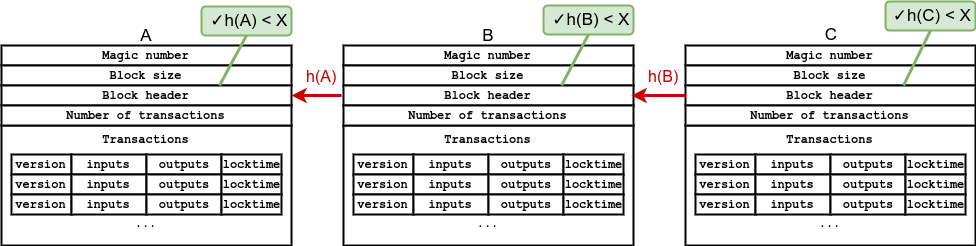
\includegraphics[width=\textwidth, height=0.8\textheight, keepaspectratio]{img/basic_blockchain_consensus.png}
 \end{exampleblock}
\end{frame}
% % % The client
\begin{frame}
 \begin{center}
  \textbf{How to handle everything?}
 \end{center}
\end{frame}
\begin{frame}{The Bitcoin client}
 \begin{block}{A Bitcoin client}
  Software that allows to operate on the Bitcoin network, handling all data structures and network messages
 \end{block}
 \pause
 \begin{block}{Features}
  \begin{enumerate}[<+->]
   \item Receive and broadcasts messages (transactions, blocks, ...)
   \item Stores and shares the \textit{blockchain}
   \item Handles keys and creates payment transactions
  \end{enumerate}
  \pause
  *Feature (2) just in \textbf{full-nodes}
 \end{block}
 \pause
 \begin{exampleblock}{Most used client}
  Bitcoin Core (\url{bitcoin.org}) is the most used Bitcoin client (\textbf{85\%} of nodes in the network)
 \end{exampleblock}
\end{frame}
% % % The problem: scalability
\begin{frame}
 \begin{center}
  \textbf{What is the limit of the technology?}
 \end{center}
\end{frame}
\subsection{The scalability problem}
\begin{frame}{Blockchain size}
 \uncover<1-2>{
  \begin{center}
   Blockchain size over time (KBytes/years)\\
   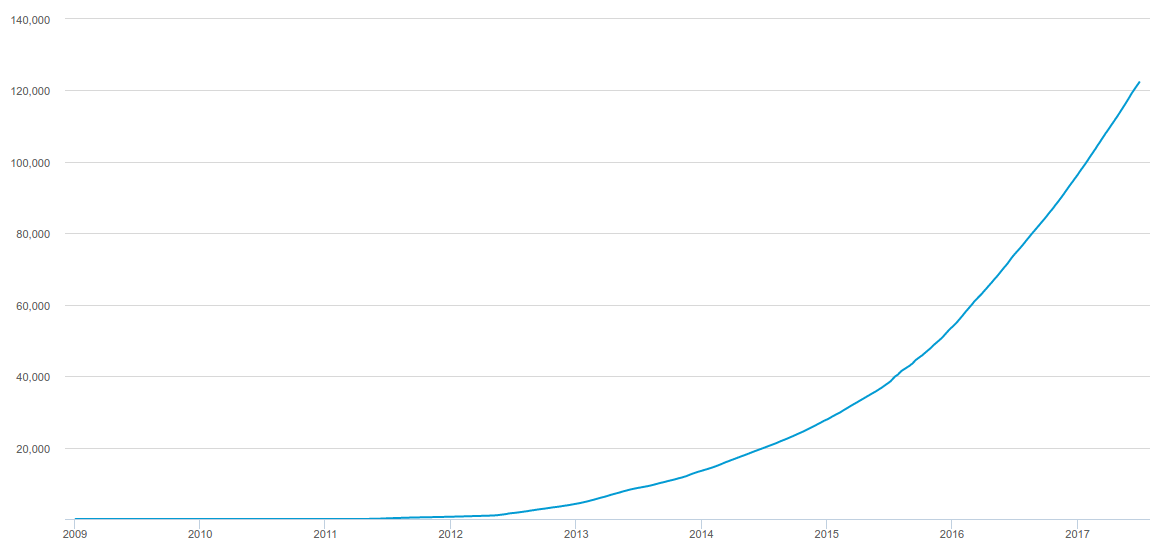
\includegraphics[width=\textwidth, height=0.8\textheight, keepaspectratio]{img/chart_blockchain_size.png}
  \end{center}
 }
 \only<2>{
  \begin{center}
   Current blockchain size is approximately \textbf{120GB}
  \end{center}
 }
 \only<3>{
  \begin{alertblock}{Increasing transaction demand}
   As Bitcoin becomes more popular, more users arrive therefore more transactions need to be processed
  \end{alertblock}}
\end{frame}
\begin{frame}{Transaction throughput}
 \begin{block}{Throughput limits}
  Because of the protocol, blocks must
  \pause
  \begin{enumerate}[<+->]
   \item \textbf{Appear every 10 minutes} (approximately) due to \textit{proof-of-work} difficulty adjustment
   \item \textbf{1MB maximum block size} to control the \textit{blockchain} growth rate
  \end{enumerate}
 \end{block}
\end{frame}
\begin{frame}{Transaction throughput}
 \begin{center}
  Transactions per block over time (tx amount/years)\\
  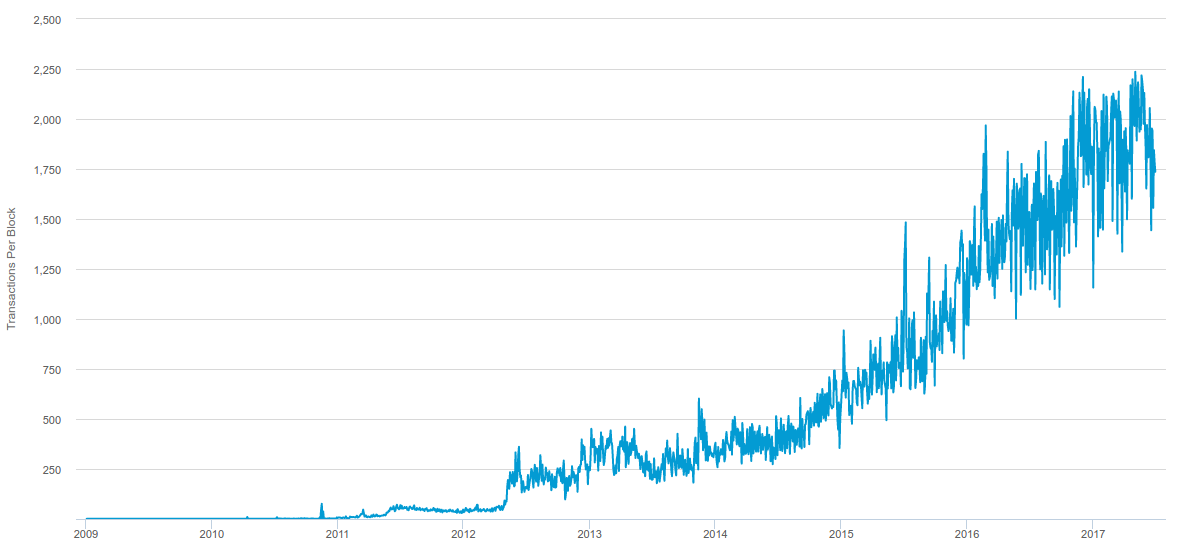
\includegraphics[width=\textwidth, height=0.8\textheight, keepaspectratio]{img/chart_block_transactions.png}
 \end{center}
 \pause
 \begin{center}
  Approximately \textbf{2.000} transactions per block
 \end{center}
\end{frame}
\begin{frame}{Transaction throughput}
 \begin{block}{Bitcoin's transaction throughput}
  Using previous information:
  \pause
  \begin{displaymath}
   \frac{2.000\ tx}{1\ block} \times \pause
   \frac{1\ block}{10\ minutes} \times \pause
   \frac{1\ minute}{60\ sec.} \approx \pause
  \end{displaymath}
  \begin{center}
   \textbf{3 transactions per second}
  \end{center}
 \end{block}
 \pause
 \begin{block}{VISA's transaction throughput}
  According to an IBM's studio performed in August of 2010:\pause
  \begin{center}
   \textbf{24.000 transactions per second}
  \end{center}
 \end{block}
\end{frame}
\begin{frame}
 \begin{center}
  \textbf{What can we do?}
 \end{center}
\end{frame}
\begin{frame}{Scalability solutions}
 \begin{center}
  Several solutions have been proposed:\\
  \pause
  \begin{enumerate}[<+->]
   \item \textbf{Increase block size}: Bitcoin Unlimited (1 to 8 MB)
   \item \textbf{Reduce transaction size}: \url{SegWit.co} (do not store transaction signatures, also fixes malleability issues)
   \item \textbf{Decrease the demand of transactions}: Payment channels
  \end{enumerate}
 \end{center}
\end{frame}
\section{Bitcoin \& Smart Contracts}
\subsection{Transactions at low-level detail}
\begin{frame}{Transactions}
 \uncover<1-5>{
  \begin{block}{Transaction fields}
   Fields of a transaction are:
   \begin{itemize}[<+->]
    \item \texttt{version}
    \item \textbf{\texttt{inputs}}
    \item \textbf{\texttt{outputs}}
    \item \texttt{locktime}
   \end{itemize}
  \end{block}}
 \only<5>{
  \begin{exampleblock}{Basic Bitcoin transaction}
   \begin{center}
    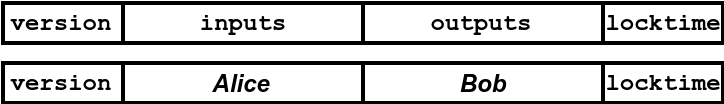
\includegraphics[width=\textwidth, height=0.8\textheight, keepaspectratio]{img/basic_tx.png}
   \end{center}
  \end{exampleblock}}
 \only<6>{
  \begin{block}{Extra "fields"}
   All transactions have an id (also called \textit{txId}), that is the
   double SHA-256 hash of the transaction bytes
  \end{block}}
\end{frame}
\begin{frame}
 \begin{center}
  \textbf{How are inputs and outputs specified?}
 \end{center}
\end{frame}
\begin{frame}{Inputs specification}
 \begin{block}{Input fields}
  An input consists of the following fields:
  \pause
  \begin{enumerate}[<+->]
   \item \textbf{previousOutput*}: An output to be spent (combination of a \textit{txId} and output number)
   \item \textbf{scriptSig}: Script necessary to authorize the output spend
   \item \textbf{sequence}: Number of the transaction in order to enable replacements
  \end{enumerate}
  \pause
  * output must not be spent by any other transaction (also called UTXO)
 \end{block}
\end{frame}
\begin{frame}{Inputs specification}
 \begin{exampleblock}{Basic transaction's input's fields}
  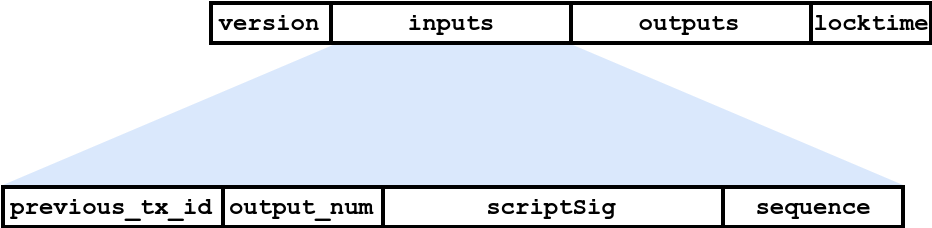
\includegraphics[width=\textwidth, height=0.8\textheight, keepaspectratio]{img/tx_input.png}
 \end{exampleblock}
\end{frame}
\begin{frame}{Outputs specification}
 \begin{block}{Output fields}
  An output consists of the following fields:
  \pause
  \begin{enumerate}[<+->]
   \item \textbf{value}: number of currency units to be sent to the output
   \item \textbf{scriptPubKey}: Script specificating the conditions for the output to be spent
  \end{enumerate}
 \end{block}
 \pause
 \begin{exampleblock}{Basic transaction's output's fields}
  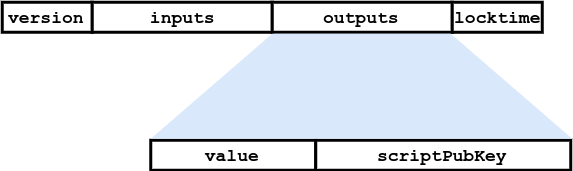
\includegraphics[width=\textwidth, height=0.8\textheight, keepaspectratio]{img/tx_output.png}
 \end{exampleblock}
\end{frame}
\begin{frame}
 \begin{center}
  \textbf{How do the scripts work?}
 \end{center}
\end{frame}
\subsection{Bitcoin's scripting language}
\begin{frame}{Bitcoin's scripting}
 \begin{block}{Bitcoin scripting language}
  Specificic scripting language for Bitcoin protocol (in transactions)
  \begin{itemize}[<+->]
   \item Simple
   \item Stack-based (processed from left to right)
   \item Purposefully not Turing-complete (with no loops)
  \end{itemize}
 \end{block}
 \pause
 \begin{block}{Technically}
  Sequentially read 1-byte opcodes that can perform arithmetical operations, store data into the stack, cryptographic operations and some logic and flow control operations
 \end{block}
\end{frame}
\begin{frame}{Transactions and scripts}
 \begin{block}{Transactions validity}
  In order for a transaction to be valid it must:
  \begin{enumerate}[<+->]
   \item \textbf{Valid inputs}: Inputs must refer to existing and non-spent outputs (UTXO)
   \item \textbf{Valid amounts}: Outputs' amounts must be less or equal to the inputs amounts
   \item \textbf{Valid scripts}: The input script followed by the output script referred by the input must execute succesfully and leave a non-empty stack
  \end{enumerate}
 \end{block}
\end{frame}
\begin{frame}{Standard scripts: P2PKH}
 \begin{block}{P2PKH: \textit{pay-to-public-key-hash}}
  The output script (\textit{scriptPubKey}) requires the input script (\textit{scriptSig}) to specify a public key whose hash matches the specified and sign the spending transaction with that public key
 \end{block}
 \pause
 \begin{exampleblock}{P2PKH sample}
  \begin{itemize}
   \visible<3->{\item \textbf{scriptSig}: \texttt{<signature> <pubKey>}}
   \visible<2->{\item \textbf{scriptPubKey}: \texttt{OP\_DUP OP\_HASH160 <pubKeyHash> OP\_EQUALVERIFY OP\_CHECKSIG}}
  \end{itemize}
 \end{exampleblock}
\end{frame}
\begin{frame}{Standard scripts: P2SH}
 \begin{block}{P2SH: \textit{pay-to-script-hash}}
  The output script (\textit{scriptPubKey}) requires the input script (\textit{scriptSig}) to specify a \textbf{redeem script} that succesfully executes and whose hash matches the specified one
 \end{block}
 \pause
 \begin{exampleblock}{P2SH sample}
  \begin{itemize}
   \visible<3->{\item \textbf{scriptSig}: \texttt{[<data>] <redeemScript>}}
   \visible<2->{\item \textbf{scriptPubKey}: \texttt{OP\_HASH160 <redeemScript\_hash> OP\_EQUAL}}
  \end{itemize}
 \end{exampleblock}
\end{frame}
\begin{frame}{Smart Contracts}
 \begin{block}{Smart Contracts}
  Computer protocols intended to facilitate, verify or enforce the negotiation or performance of a contract
 \end{block}
 \pause
 \begin{block}{Smart Contracts in Bitcoin}
  Creation of \textit{redeemScripts} redeemable using P2SH script sets in transactions.
  \pause
  \begin{center}
   \textbf{\textit{redeemScripts} are Bitcoin's smart contracts}
  \end{center}
 \end{block}
\end{frame}
\begin{frame}
 \begin{center}
  \textbf{What can we do with Smart Contracts?}\\
  \pause
  \huge\textbf{Payment channels}
 \end{center}
\end{frame}
\subsection{What is a payment channel?}
\begin{frame}{What is a Payment channel?}
 \begin{block}{Payment channel}
  Set of techniques designed to allow users to make multiple Bitcoin transactions without commiting all of them to the Bitcoin block chain
 \end{block}
 \pause
 \begin{block}{\textit{Off-chain} transactions}
  Bitcoin transactions that are not commited to the Bitcoin blockchain but would be valid if they were commited
 \end{block}
\end{frame}
\begin{frame}{Payment Channel basic scheme}
 \begin{block}{Scheme}
  All payment channels follow a basic scheme:
  \pause
  \begin{enumerate}[<+->]
   \item \textbf{Funding:} Some funds are locked so they can be moved with payments during the channel operation
   \item \textbf{Payment:} Locked funds are moved to pay to a party of the channel
   \item \textbf{Closure:} Funds are unlocked and returned to the channel parties with the final balance after all payments
  \end{enumerate}
 \end{block}
 \pause
 \begin{block}{Which transactions are \textit{off-chain}?}
  \begin{center}
   All \textbf{payment transactions are \textit{off-chain}}
  \end{center}
 \end{block}
\end{frame}
\section{Unidirectional payment channels}
\begin{frame}
 \begin{center}
  \textbf{What does a unidirectional payment channel allows us to do?}\\
 \end{center}
\end{frame}
\begin{frame}{Unidirectional payment channel}
 \begin{block}{What allows to do?}
  Incrementally pay amounts of funds from one party to another
 \end{block}
 \pause
 \begin{exampleblock}{For instance...}
  We will create a channel to allow \textbf{Alice} pay \textbf{Bob} incremental amounts of funds
 \end{exampleblock}
\end{frame}
\subsection{Scheme}
\begin{frame}{Locking funds}
 \begin{block}{What do we need to do?}
  Lock funds into the channel so:
  \pause
  \begin{enumerate}[<+->]
   \item \textbf{Both} must authorize a payment:
         \begin{itemize}[<+->]
          \item Alice must want to pay some amount to Bob (Bob can not pay hisself)
          \item Bob must authorize payments in order to check funds are send to him (and not to Alice)
         \end{itemize}
   \item \textbf{Refunds} must be possible if a party does not cooperate
  \end{enumerate}
 \end{block}
 \pause
 \begin{block}{How to refund}
  Lock the funds for an amount of time, so after that time (called the \textit{channel expiry time}) the funds are given back to the funder
 \end{block}
\end{frame}
\begin{frame}{Locking funds}
 \begin{block}{Ways to lock funds}
  In order to accomplish both properties to lock funds, we can:
  \pause
  \begin{enumerate}[<+->]
   \item Create a \textbf{funding transaction} and a time-locked \textbf{refund transaction}
   \item Create a \textbf{\textit{smart} funding transaction} with
         the time-lock integrated in the \textit{smart contract}
  \end{enumerate}
 \end{block}
\end{frame}
\begin{frame}{Paying funds}
 \begin{block}{What do we need to do?}
  In order to create a payment transaction, as both users must authorize payments:
  \pause
  \begin{enumerate}[<+->]
   \item \textbf{Alice} creates and signs a transaction paying some of the locked funds to \textbf{Bob} (and the rest to Alice as return)
   \item \textbf{Bob} stores the partially signed transaction that pays some amount of money to him
   \item If \textbf{Alice} wants to pay more, repeats the first step with more funds (spending the same funding transaction)
  \end{enumerate}
 \end{block}
 \pause
 \begin{block}{Replace by economical incentive}
  Bob will \textbf{keep the latest payment transaction} and discard previous ones, as \textbf{the last will be the one that pays more to him}
 \end{block}
\end{frame}
\begin{frame}{Closure}
 \begin{block}{What do we need to do?}
  Two situations can appear when closing the channel:
  \begin{enumerate}[<+->]
   \item \textbf{Graceful closure}: the channel has been operated and the expiry time is close, so \textbf{latest payment transaction is broadcasted}, spending the funding transaction and closing the channel.
   \item \textbf{No cooperation}: if Bob disappears, Alice will \textbf{broadcast a refund transaction} to recover the locked funds
  \end{enumerate}
 \end{block}
\end{frame}
\subsection{Implementation}
\begin{frame}{Locking the funds}
 \begin{block}{Ways to lock funds}
  In order to accomplish both properties to lock funds, we can:
  \begin{enumerate}
   \item Create a \textbf{funding transaction} and a time-locked \textbf{refund transaction}
   \item Create a \textbf{\textit{smart} funding transaction} with
         the time-lock integrated in the \textit{smart contract}
  \end{enumerate}
 \end{block}
 \pause
 \begin{block}{The implementation}
  With the \textbf{BIP-65}, an opcode appeared to create time-locked smart contracts, so we can create a \textbf{\textit{smart} funding transaction} with the time lock integrated
 \end{block}
\end{frame}
\begin{frame}{Funding transaction}
 \begin{exampleblock}{Funding transaction}
  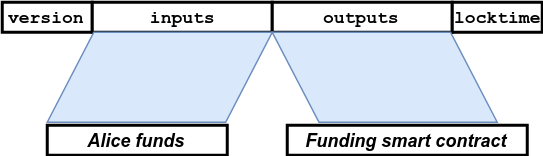
\includegraphics[width=\textwidth, height=0.8\textheight, keepaspectratio]{img/unidir_tx_funding.png}
 \end{exampleblock}
 \pause
\end{frame}
\begin{frame}{Funding transaction}
 \begin{exampleblock}{Funding smart contract}
  As we said, we need to design a \textit{redeemScript} in order to create a Bitcoin smart contract:
  \pause
  \begin{center}
   \texttt{OP\_IF <time>}\\
   \texttt{OP\_CHECKLOCKTIMEVERIFY OP\_DROP <PubKeyAlice\_1> OP\_CHECKSIG}\\
   \texttt{OP\_ELSE}\\
   \texttt{OP\_2 <PubKeyAlice\_2> <PubKeyBob> OP\_2 OP\_CHECKMULTISIG OP\_ENDIF}
  \end{center}
 \end{exampleblock}
 \pause
 \begin{exampleblock}{Technically...}
  As we are creating a P2SH, then the output script must be:\
  \texttt{OP\_HASH160 <redeemScript\_hash> OP\_EQUAL}
 \end{exampleblock}
\end{frame}
\begin{frame}{Paying funds}
 \begin{block}{What do we need to do?}
  In order to create a payment transaction, as both users must authorize payments:
  \begin{enumerate}
   \item \textbf{Alice} creates and signs a transaction paying some of the locked funds to \textbf{Bob} (and the rest to Alice as return)
   \item \textbf{Bob} stores the partially signed transaction that pays some amount of money to him
   \item If \textbf{Alice} wants to pay more, repeats the first step with more funds (spending the same funding transaction)
  \end{enumerate}
 \end{block}
 \pause
 \begin{block}{The implementation}
  Alice creates a transaction that spends the funding transaction, with two outputs: one with some amount for Bob and the rest for herself
 \end{block}
\end{frame}
\begin{frame}{Payment transaction}
 \begin{exampleblock}{Payment transaction}
  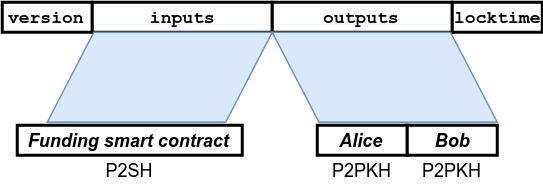
\includegraphics[width=\textwidth, height=0.8\textheight, keepaspectratio]{img/unidir_tx_payment.png}
 \end{exampleblock}
\end{frame}
\begin{frame}{Payment transaction}
 \begin{exampleblock}{Spending funding smart contract}
  We now need to spend the \textit{redeemScript}
  \pause
  \begin{center}
   \texttt{OP\_0 <sig\_Alice> <sig\_Bob> OP\_0}
  \end{center}
 \end{exampleblock}
 \begin{exampleblock}{Technically...}
  As we are spending a P2SH, then the input script must be:\
  \texttt{OP\_0 <sig\_Alice> <sig\_Bob> OP\_0 <redeemScript>}
 \end{exampleblock}
\end{frame}
\begin{frame}{Closure transaction}
 \begin{block}{What do we need to do?}
  Two situations can appear when closing the channel:
  \begin{enumerate}[<+->]
   \item \textbf{Graceful closure}: the channel has been operated and the expiry time is close, so \textbf{latest payment transaction is broadcasted}, spending the funding transaction and closing the channel.
   \item \textbf{No cooperation}: if Bob disappears, Alice will \textbf{broadcast a refund transaction} to recover the locked funds
  \end{enumerate}
 \end{block}
 \pause
 \begin{exampleblock}{Graceful closure}
  Bob simply broadcasts the latest payment transaction once signed and before channel expiry time
 \end{exampleblock}
\end{frame}
\begin{frame}{Closure transaction}
 \begin{exampleblock}{Closure transaction (refund)}
  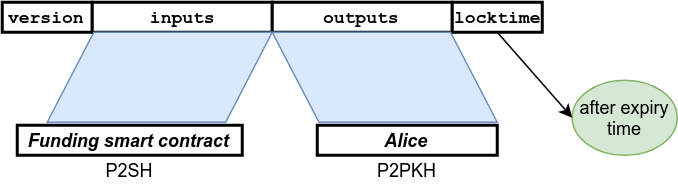
\includegraphics[width=\textwidth, height=0.8\textheight, keepaspectratio]{img/unidir_tx_refund.png}
 \end{exampleblock}
\end{frame}
\begin{frame}{Closure transaction}
 \begin{exampleblock}{Spending funding smart contract (refund)}
  We now need to spend the \textit{redeemScript} after the lock time
  \pause
  \begin{center}
   \texttt{<sig\_Alice> OP\_1}
  \end{center}
 \end{exampleblock}
 \pause
 \begin{exampleblock}{Technically...}
  As we are spending a P2SH, then the input script must be:\
  \texttt{<sig\_Alice> OP\_1 <redeemScript>}
 \end{exampleblock}
\end{frame}
\begin{frame}
 \begin{center}
  \textbf{What if we want Bob to pay Alice too?}
 \end{center}
\end{frame}
\section{Bidirectional payment channels}
\begin{frame}{Bidirectional payment channel}
 \begin{block}{What allows to do?}
  Incrementally pay amounts of funds from one party to another \textbf{and viceversa}
 \end{block}
 \pause
 \begin{exampleblock}{For instance...}
  We will create a channel to allow \textbf{Alice} pay \textbf{Bob} incremental amounts of funds \textbf{and viceversa}
 \end{exampleblock}
\end{frame}
\subsection{Scheme}
\begin{frame}{Bidirectional payment channels' scheme}
 \begin{block}{Source}
  Obtained from
  \begin{quote}
   A Fast and Scalable Payment Network with Bitcoin Duplex Micropayment Channels - \textit{Christian Decker \& Roger Wattenhofer}
  \end{quote}
 \end{block}
 \pause
 \begin{block}{Idea}
  Use \textbf{two unidirectional channels}, one in each way with an \textbf{invalidation tree} to perform resets
 \end{block}
\end{frame}
\subsection{Implementation}
\begin{frame}{Locking the funds}
 \begin{block}{Ways to lock funds}
  In order to accomplish both properties to lock funds, we can:
  \begin{enumerate}
   \item Create a \textbf{funding transaction} and a time-locked \textbf{refund transaction}
   \item Create a \textbf{\textit{smart} funding transaction} with
         the time-lock integrated in the \textit{smart contract}
  \end{enumerate}
 \end{block}
 \pause
 \begin{block}{The implementation}
  We can still use \textbf{BIP-65} to create a time-locking smart contract
 \end{block}
\end{frame}
\begin{frame}{Funding transaction}
 \begin{exampleblock}{Funding transaction}
  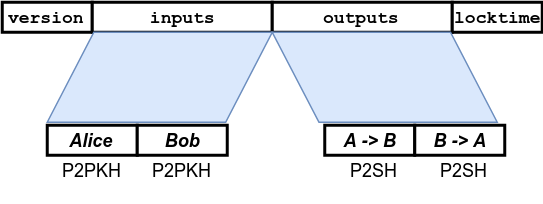
\includegraphics[width=\textwidth, height=0.8\textheight, keepaspectratio]{img/bidir_tx_funding.png}
 \end{exampleblock}
\end{frame}
\begin{frame}{Funding transaction}
 \begin{exampleblock}{Funding smart contract}
  Same as unidirectional channel, but with two outputs
  \pause
  \begin{center}
   \begin{enumerate}[<+->]
    \item \textbf{Alice to Bob output}\\
          \small{\texttt{OP\_IF <time> OP\_CHECKLOCKTIMEVERIFY OP\_DROP <PubKeyAlice\_1> OP\_CHECKSIG OP\_ELSE OP\_2 <PubKeyAlice\_2> <PubKeyBob\_1> OP\_2 OP\_CHECKMULTISIG OP\_ENDIF}}
    \item \textbf{Bob to Alice output}\\
          \small{\texttt{OP\_IF <time> OP\_CHECKLOCKTIMEVERIFY OP\_DROP <PubKeyBob\_2> OP\_CHECKSIG OP\_ELSE OP\_2 <PubKeyAlice\_3> <PubKeyBob\_3> OP\_2 OP\_CHECKMULTISIG OP\_ENDIF}}
   \end{enumerate}
  \end{center}
 \end{exampleblock}
 \pause
 \begin{exampleblock}{Technically...}
  As we are creating a P2SH, then the outputs' script must be:\
  \texttt{OP\_HASH160 <redeemScript\_hash> OP\_EQUAL}
 \end{exampleblock}
\end{frame}
\begin{frame}{Paying funds}
 \begin{block}{What do we need to do?}
  In order to create a payment transaction, as both users must authorize payments:
  \begin{enumerate}
   \item \textbf{Alice} creates and signs a transaction paying some of the locked funds to \textbf{Bob} (and the rest to Alice as return)
   \item \textbf{Bob} stores the partially signed transaction that pays some amount of money to him
   \item If \textbf{Alice} wants to pay more, repeats the first step with more funds (spending the same funding transaction)
  \end{enumerate}
 \end{block}
 \pause
 \begin{block}{The implementation}
  Same of a unidirectional payment channel, but Bob can pay Alice too using his channel
 \end{block}
\end{frame}
\begin{frame}{Payment transaction}
 \begin{exampleblock}{Payment transaction}
  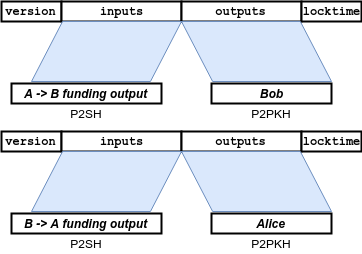
\includegraphics[width=\textwidth, height=0.8\textheight, keepaspectratio]{img/bidir_tx_payment.png}
 \end{exampleblock}
\end{frame}
\begin{frame}{Payment transaction}
 \begin{exampleblock}{Spending funding smart contract}
  We now need to spend the \textit{redeemScript}
  \pause
  \begin{center}
   \begin{enumerate}[<+->]
    \item \textbf{Alice to Bob output}\\
          \small{\texttt{OP\_0 <sig\_Alice> <sig\_Bob> OP\_0}}
    \item \textbf{Bob to Alice output}\\
          \small{\texttt{OP\_0 <sig\_Alice> <sig\_Bob> OP\_0}}
   \end{enumerate}
  \end{center}
 \end{exampleblock}
 \begin{exampleblock}{Technically...}
  As we are spending a P2SH, then the input script must be:\
  \texttt{OP\_0 <sig\_Alice> <sig\_Bob> OP\_0 <redeemScript>}
 \end{exampleblock}
\end{frame}
\begin{frame}{Closure transaction}
 \begin{block}{What do we need to do?}
  Two situations can appear when closing the channel:
  \begin{enumerate}
   \item \textbf{Graceful closure}: the channel has been operated and the expiry time is close, so \textbf{latest payment transaction \underline{of each output} is broadcasted}, spending the funding transaction and closing the channel.
   \item \textbf{No cooperation}: if any of the parties do not cooperate, they can \textbf{broadcast a refund transaction} to recover their locked funds
  \end{enumerate}
 \end{block}
 \pause
 \begin{exampleblock}{Graceful closure}
  Alice and Bob simply broadcast the latest payment transaction once signed and before channel expiry time
 \end{exampleblock}
\end{frame}
\begin{frame}{Closure transaction}
 \begin{exampleblock}{Closure transaction (refund)}
  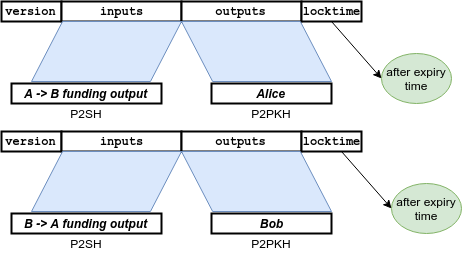
\includegraphics[width=\textwidth, height=0.8\textheight, keepaspectratio]{img/bidir_tx_refund.png}
 \end{exampleblock}
\end{frame}
\begin{frame}{Closure transaction}
 \begin{exampleblock}{Spending funding smart contract (refund)}
  We now need to spend the \textit{redeemScript} after the lock time
  \pause
  \begin{center}
   \begin{enumerate}[<+->]
    \item \textbf{Alice to Bob output refund}\\
          \texttt{<sig\_Alice> OP\_1}
    \item \textbf{Bob to Alice output refund}\\
          \texttt{<sig\_Bob> OP\_1}
   \end{enumerate}
  \end{center}
 \end{exampleblock}
 \pause
 \begin{exampleblock}{Technically...}
  As we are spending a P2SH, then the input script must be:\
  \texttt{<sig\_Alice|Bob> OP\_1 <redeemScript>}
 \end{exampleblock}
\end{frame}
\subsection{Problem: channel reseting}
\begin{frame}
 \begin{center}
  \textbf{What if one of the payment channels gets exhausted?}\\
  \pause
  \huge\textbf{Channel resetting}
 \end{center}
\end{frame}
\begin{frame}{Channel resetting}
 \begin{exampleblock}{A simple reset example}
  \begin{center}
   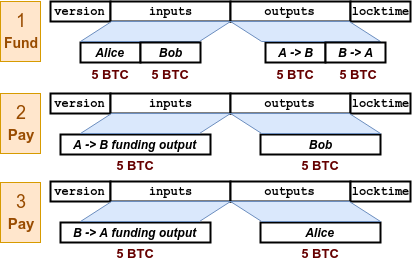
\includegraphics[width=\textwidth, height=0.8\textheight, keepaspectratio]{img/bidir_reset.png}
  \end{center}
 \end{exampleblock}
\end{frame}
\begin{frame}{Channel resetting}
 \begin{alertblock}
  Both parties own the same amount of funds as at the beginning of the channel but their respective payment channels have been exhausted. No more incremental payments can be performed
 \end{alertblock}
\end{frame}
\begin{frame}{Resetting by invalidation trees}
 \begin{block}{Invalidation tree}
  Tree of transactions that use the timelock field to invalidate old branches of the tree and be able to create new ones with an updated status of the balances
 \end{block}
 \pause
 \begin{block}{Replace by timelock}
  Create timelocked transactions so that when using timelocks nearer to the present invalidate transactions with later timelocks
 \end{block}
\end{frame}
\begin{frame}{An invalidation tree reset example}
 \begin{exampleblock}{Reset by adding a new leaf}
  \begin{center}
   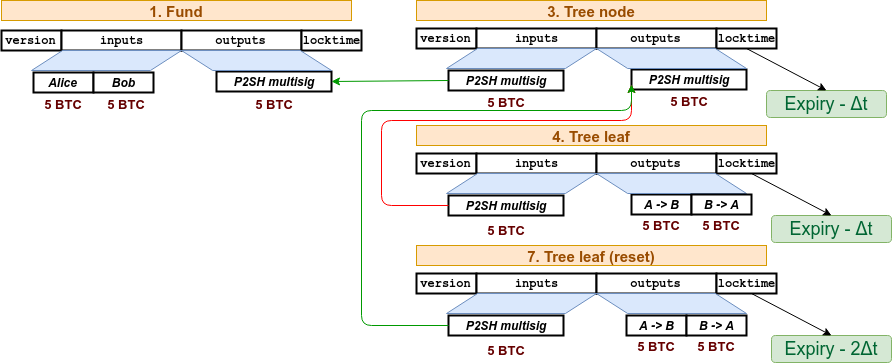
\includegraphics[width=\textwidth, height=0.8\textheight, keepaspectratio]{img/bidir_tree.png}
  \end{center}
 \end{exampleblock}
\end{frame}
\begin{frame}{An invalidation tree reset example}
 \begin{exampleblock}{Reset by branching}
  \begin{center}
   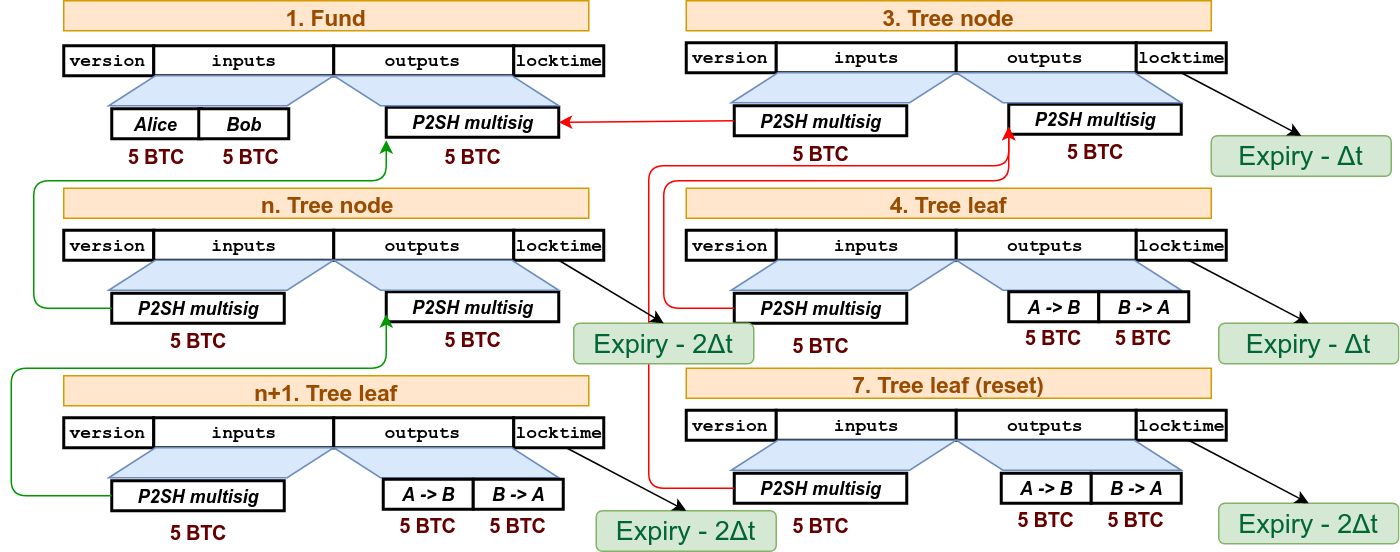
\includegraphics[width=\textwidth, height=0.8\textheight, keepaspectratio]{img/bidir_tree_expanded.png}
  \end{center}
 \end{exampleblock}
\end{frame}
\begin{frame}{Differences}
 \begin{block}{Basic duplex channel vs Resetable duplex channel}
  \begin{itemize}[<+->]
   \item \textbf{More complex to use BIP-65*}: As the tree requires linking P2SH single outputs, we can't use BIP-65 to create a timelock contract.
         \pause
         \small{*this would require to generate two outputs and inputs in each first tree node with all data required}
   \item \textbf{More transactions needed:} in order to create the tree (be careful with signing order of all parties to prevent attacks)
   \item \textbf{Reduced expiry time:} each tree branch reduces the channel's effective expiry time
  \end{itemize}
 \end{block}
\end{frame}
\begin{frame}{Pros and cons}
 \begin{exampleblock}{Pros}
  \begin{itemize}[<+->]
   \item \textbf{Simple to create}: no complex transactions needed, unlike the \textit{Lightning Network} smart contracts
   \item \textbf{No extra data exchange}: unlike the \textit{Lightning Network}, the protocol does not require to exchange secrets or additional data
  \end{itemize}
 \end{exampleblock}
 \pause
 \begin{alertblock}{Cons}
  \begin{itemize}[<+->]
   \item \textbf{Reducing expiry time}: the more resets needed, the more the effective expiry time is reduced (more invalidating branches and leafs)
   \item \textbf{Need to store more transactions}: in other solutions for duplex payment channel, like the \textit{Lightning Network}, just the latest payment transaction must be saved, and not an entire tree.
  \end{itemize}
 \end{alertblock}
\end{frame}
\section{The Bitcoin framework}
\begin{frame}{Developing problems}
 \begin{alertblock}{Problems when implementing the channel}
  \begin{itemize}[<+->]
   \item \textbf{Lack of documentation}: Bitcoin is missing from good quality, low-level protocol implementation details. Most accurate information is spread around Q\&A sites, \textit{Bitcoin Wiki} and \textit{Bitcoin Core's client} C++ code
   \item \textbf{Lack of low-level, documented libraries}: There are very few libraries that handle the Bitcoin protocol complexities (no library found to create raw transaction signatures with a customized transaction)
  \end{itemize}
 \end{alertblock}
\end{frame}
\begin{frame}{Our Bitcoin framework}
 \begin{exampleblock}{Solution: our own Bitcoin framework}
  All what we* learned was implemented in our own Bitcoin framework that has:
  \begin{itemize}
   \item \textbf{Designed for ease of use:} Everything was first designed previous to its codification using software patterns to enhace developers' usability
   \item \textbf{OOP and puzzle-friendliness principles:} All data we have learned has been coded into serializable and deserializable classes that can be joined together making the framework a modulable puzzle of Bitcoin data pieces implemented as classes
   \item \textbf{Extensive documentation:} Every file, class and method is properly commented in order to generate an understandable and extensive documentation
   \item \textbf{Extensively tested:} Every module has been tested with other libraries and with the \textit{Bitcoin Core} client, sending transactions formed with the framework to the Bitcoin's \textit{testnet}
  \end{itemize}
  \pause
  \begin{center}
   *developed along Carlos González Cebrecos
  \end{center}
 \end{exampleblock}
\end{frame}
\begin{frame}{Channel implementation}
 \begin{block}{Fork of the Bitcoin framework}
  The channel was implemented forking the framework in a script so it can be operated from the CLI passing the required parameters (funds amount, public and private keys, previous inputs, ...)
 \end{block}
 \pause
 \begin{alertblock}{Channel lacks ease of use}
  Because focused on the \textbf{channel protocol's design to enhace security}, no time was missing to automate the operatibility of the channel:
  \begin{itemize}
   \item \textbf{Bitcoin Core RPC:} to automate transaction broadcasting, UTXO detection, balance detection, fee calculation, ...
   \item \textbf{Channel state storage:} automatically store in the user's computer the state of the channel (transactions' tree and refunds)
   \item \textbf{Graphical UI:} to enable every Bitcoin user enjoy the payment channels' power
  \end{itemize}
 \end{alertblock}
\end{frame}
\section{Conclusions}
\begin{frame}
    Along this project, I've learned:
    \begin{itemize}[<+->]
        \item \textbf{Low-level understanding of the Bitcoin protocol}: By learning how to implement Smart Contracts on Bitcoin and creating the framework to ease those smart contracts creation
        \item \textbf{Bitcoin lacks of low-level extensive documentation}: Developing in Bitcoin has no formal, low-level detailed guide and most advanced features can just be learned by inspecting the \textit{Bitcoin Core} C++ code
        \item \textbf{Payment Channels are the future of Bitcoin}: Maybe \textit{Lightning Network} has a better structure and protocol implementation, but what is crystal clear is that multi-hop duplex payment channels are the Bitcoin's future after \textit{SegWit.co} activates in the \textit{mainnet} allowing a secure implementation of them.
    \end{itemize}
\end{frame}
\begin{frame}
    \begin{center}
        \textbf{\huge{Thanks for your attention}}\\
        \pause
        Q\&A round
    \end{center}
\end{frame}
\end{document}
